\documentclass[12pt,a4paper]{article}
\synctex=1
\usepackage[utf8]{inputenc}
\usepackage[margin=2cm]{geometry}
\usepackage{graphicx}
%\usepackage{verbatim}
\usepackage{listings}
\usepackage{multicol}
\usepackage{libertine}
\usepackage{pgfornament}
\usepackage{eso-pic}
\usepackage{textcomp}
\usepackage{courier}
\usepackage[hangul]{kotex}
\linespread{1.3}

\title{
	\centering
	\pgfornament[width=12cm,color=teal]{84}\\
	\vspace{1cm}
	\fontsize{50}{50} \selectfont {시스템 S/W 실습4}\\
	\pgfornament[width=12cm,color=teal]{88}\\
	\vfill}
\author{
	\LARGE
	\begin{tabular}{rl}
		\hline
		학번 : & 2016110056\\ 
		학과 : & 불교학부 \\
		이름 : & 박승원\\
		날짜 : & \today\\
		\hline
	\end{tabular}\vspace{2cm}
	\\
	\includegraphics[width=0.5\textwidth]{logo.jpg}
}
\date{}

\begin{document}
\maketitle
\noindent
\lstset{columns=flexible, tabsize=4, frame=single, showstringspaces=false, breaklines=true, upquote=true, basicstyle=\ttfamily\normal}
\begin{enumerate}


\lstset{language=C}
%\begin{multicols}{2}
\item 다음에 주어진 프로그램 내용을 편집하여 test4.c로 저장하고, test4.c를 Compile 하여 object file test4를 생성하고, 입력 data file 'srcfile'을 준비하여 test4를 실행하시오. \\
단 C Program compile 명령은 다음과 같고, test4의 입력파일 srcfile(SIC 어셈블리어 프로그램 파일)은 각자 준비한다.

\$gcc -0 test4 test.c\\
\$./test4 srcfile

\lstinputlisting[title=test4old.c]{test4old.c}

\item 위의 소오스 파일은 라벨의 길이에 제한이 있어서 좀 더 범용적으로 고쳐 보았다.

\lstinputlisting[title=test4.c]{test4.c}

\item 실행 결과
\\다음과 같은 4가지의 소오스 파일을 준비하여 실행해 보았다.
\lstinputlisting[language=asm]{ss.s}

다음과 같은 실행 결과를 얻었다.

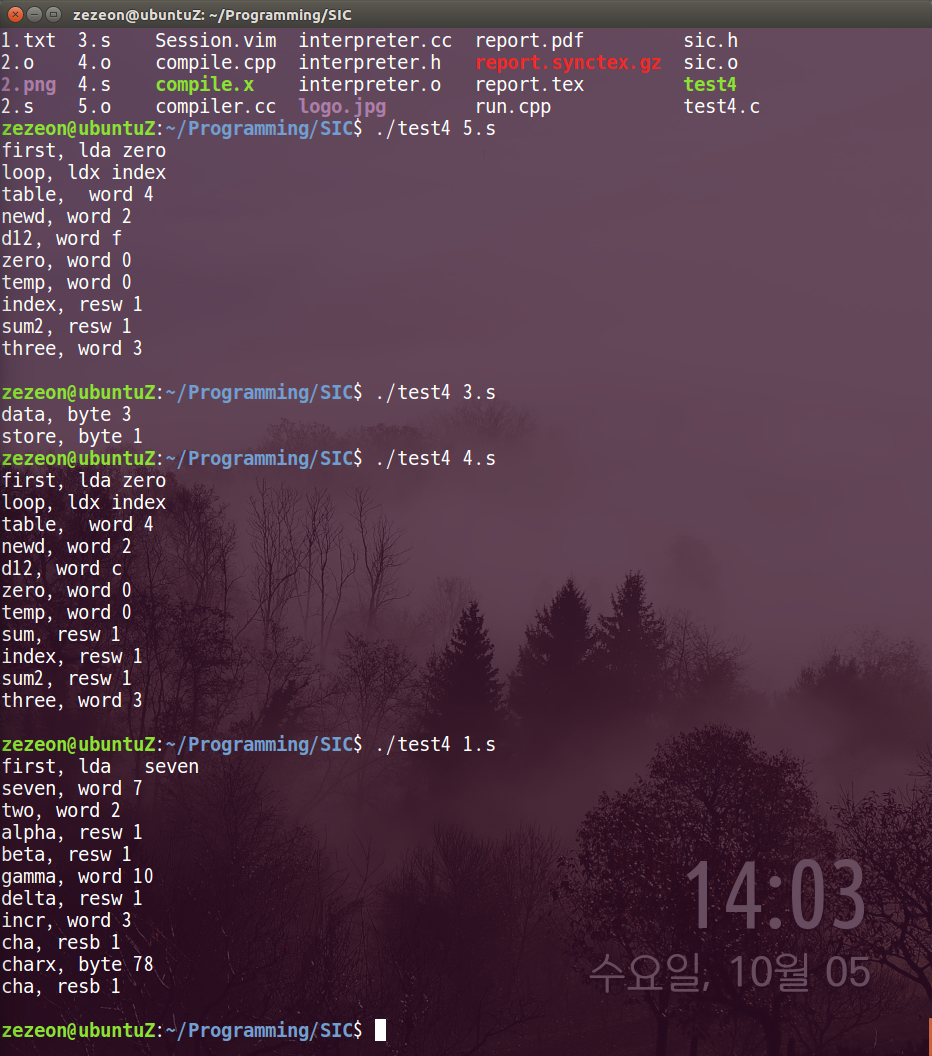
\includegraphics[width=\textwidth]{1.png}

\end{enumerate}

{\Huge소감}
\indent
실습내용이 그다지 많지 않아 7장 분량을 채우기가 힘들었다. 수업이 정상적으로 진도가 나가지 못하는 것 같아 안타깝다. 다음 주에도 쉰다니 시스템 소프트웨어는 매우 중요한 과목이라 들었는데, 교수님께서 바쁘시겠지만, 수업을 보충하는 시간을 내주시면 어떨까 하는 것이 개인적 바램입니다.
\end{document}
